\chapter{Introduction}

\begin{figure}
	\centerline{
		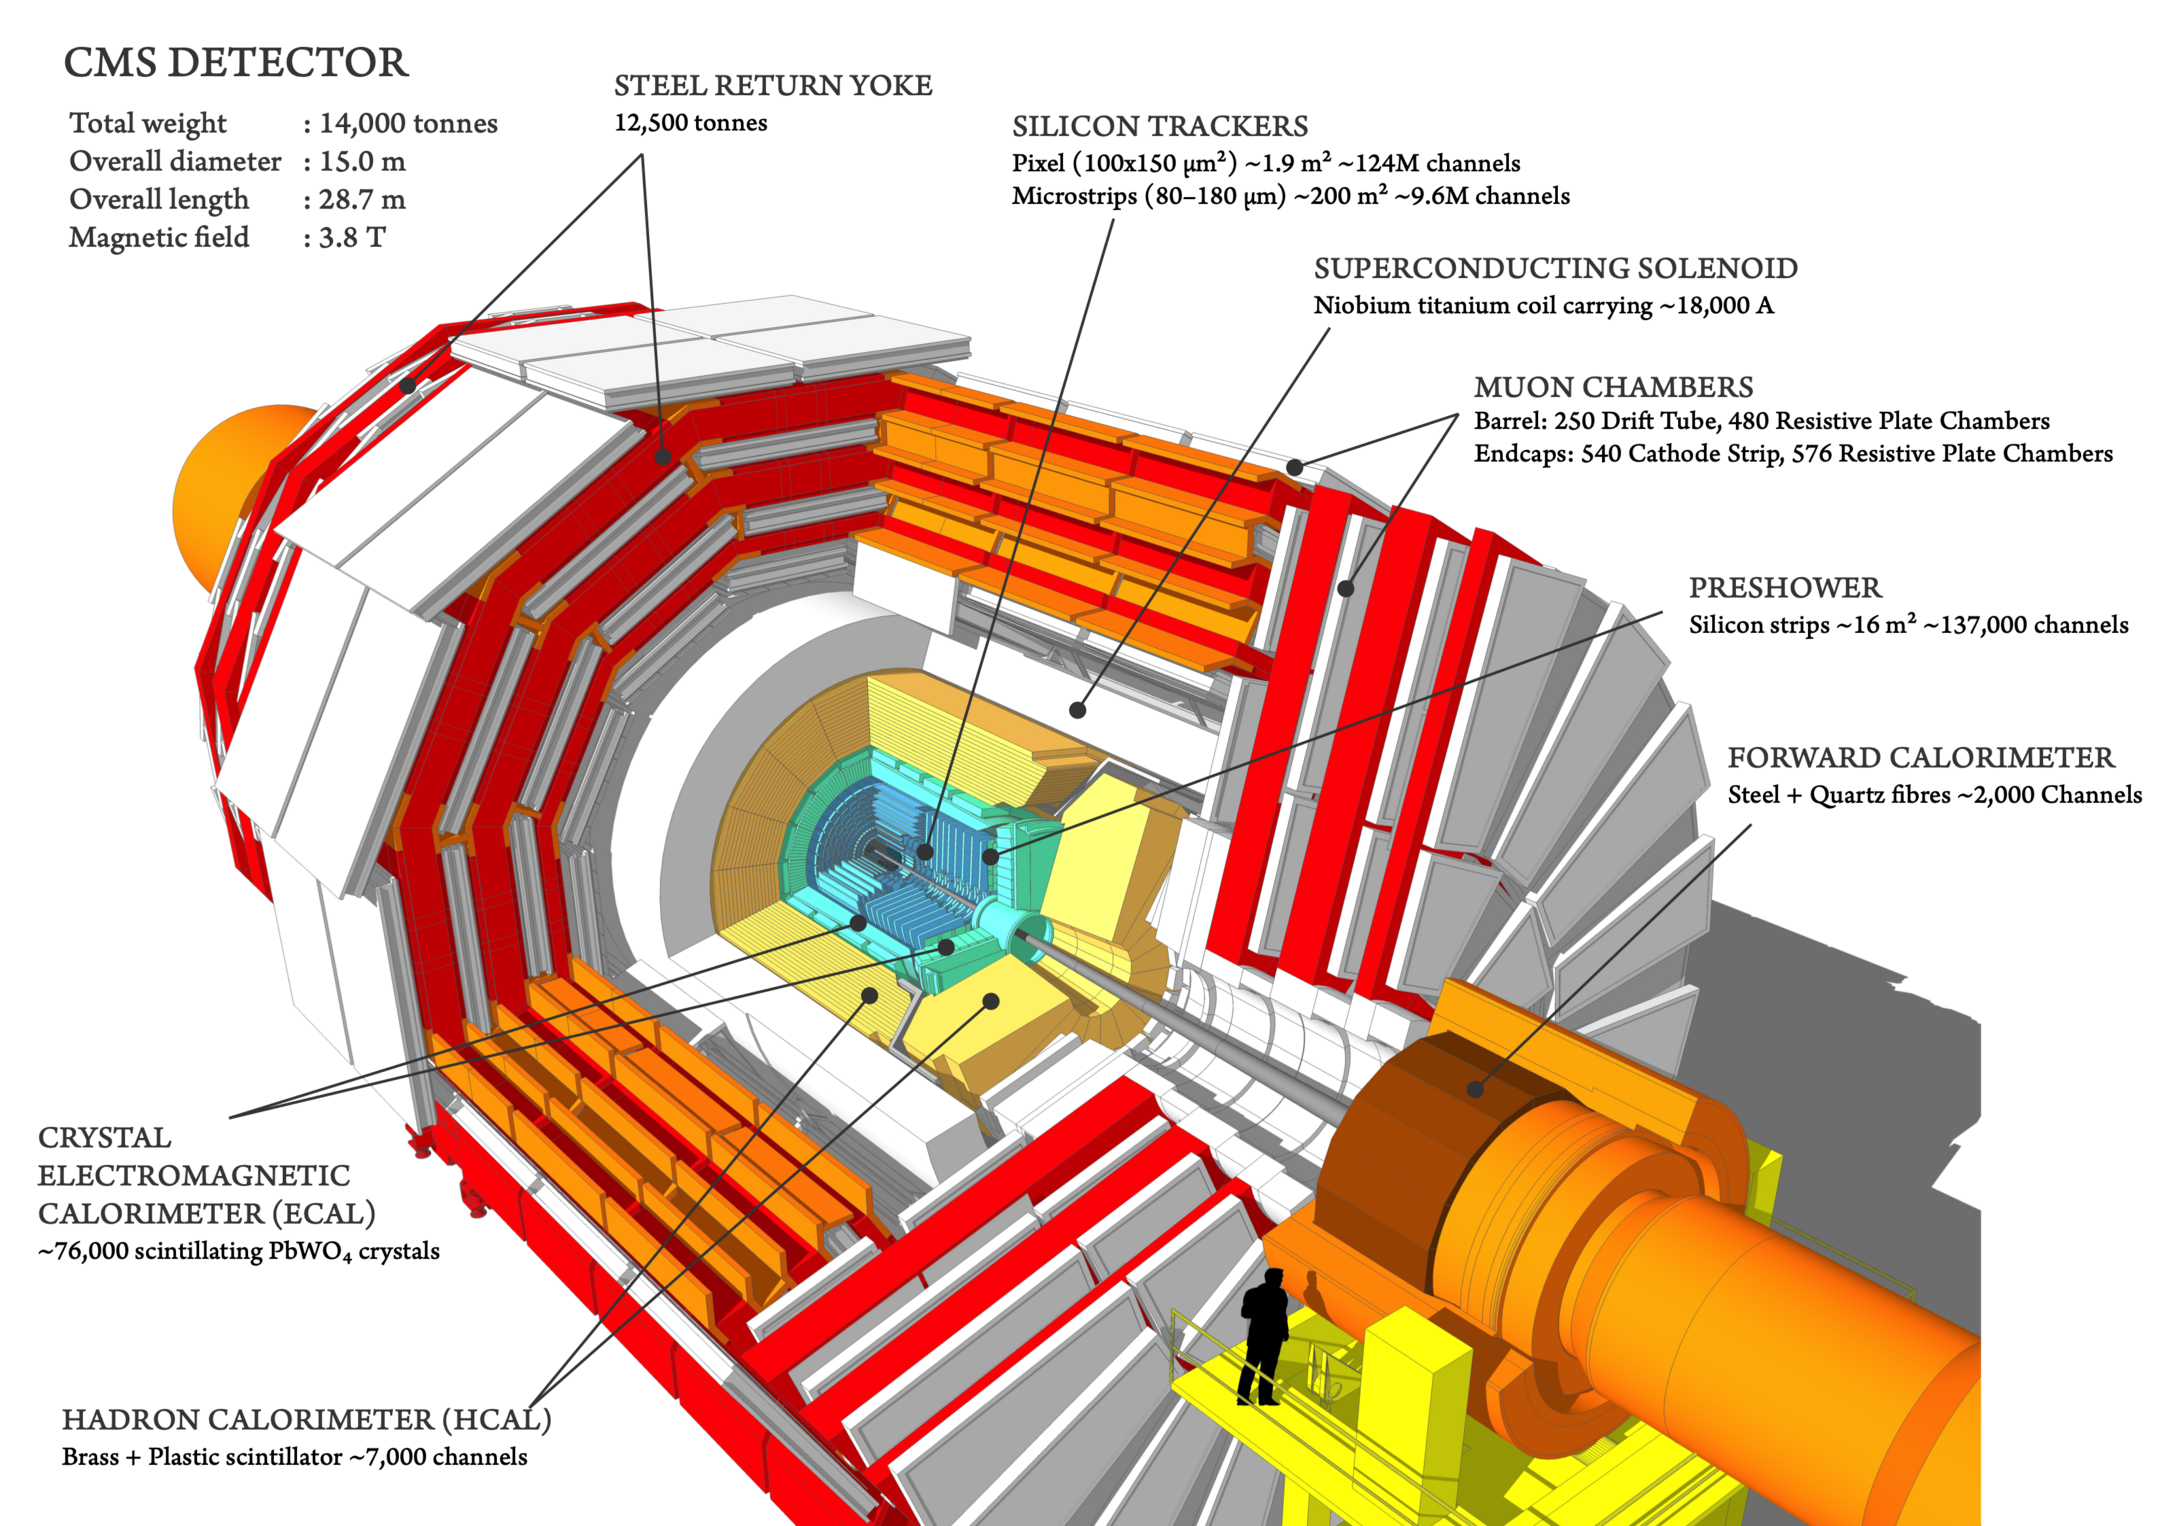
\includegraphics[width=0.8\paperwidth]{cms}}
	\caption{Cutaway diagram of the CMS detector \cite{Sakuma_2014}}

\end{figure}

\begin{figure}
	\centerline{
		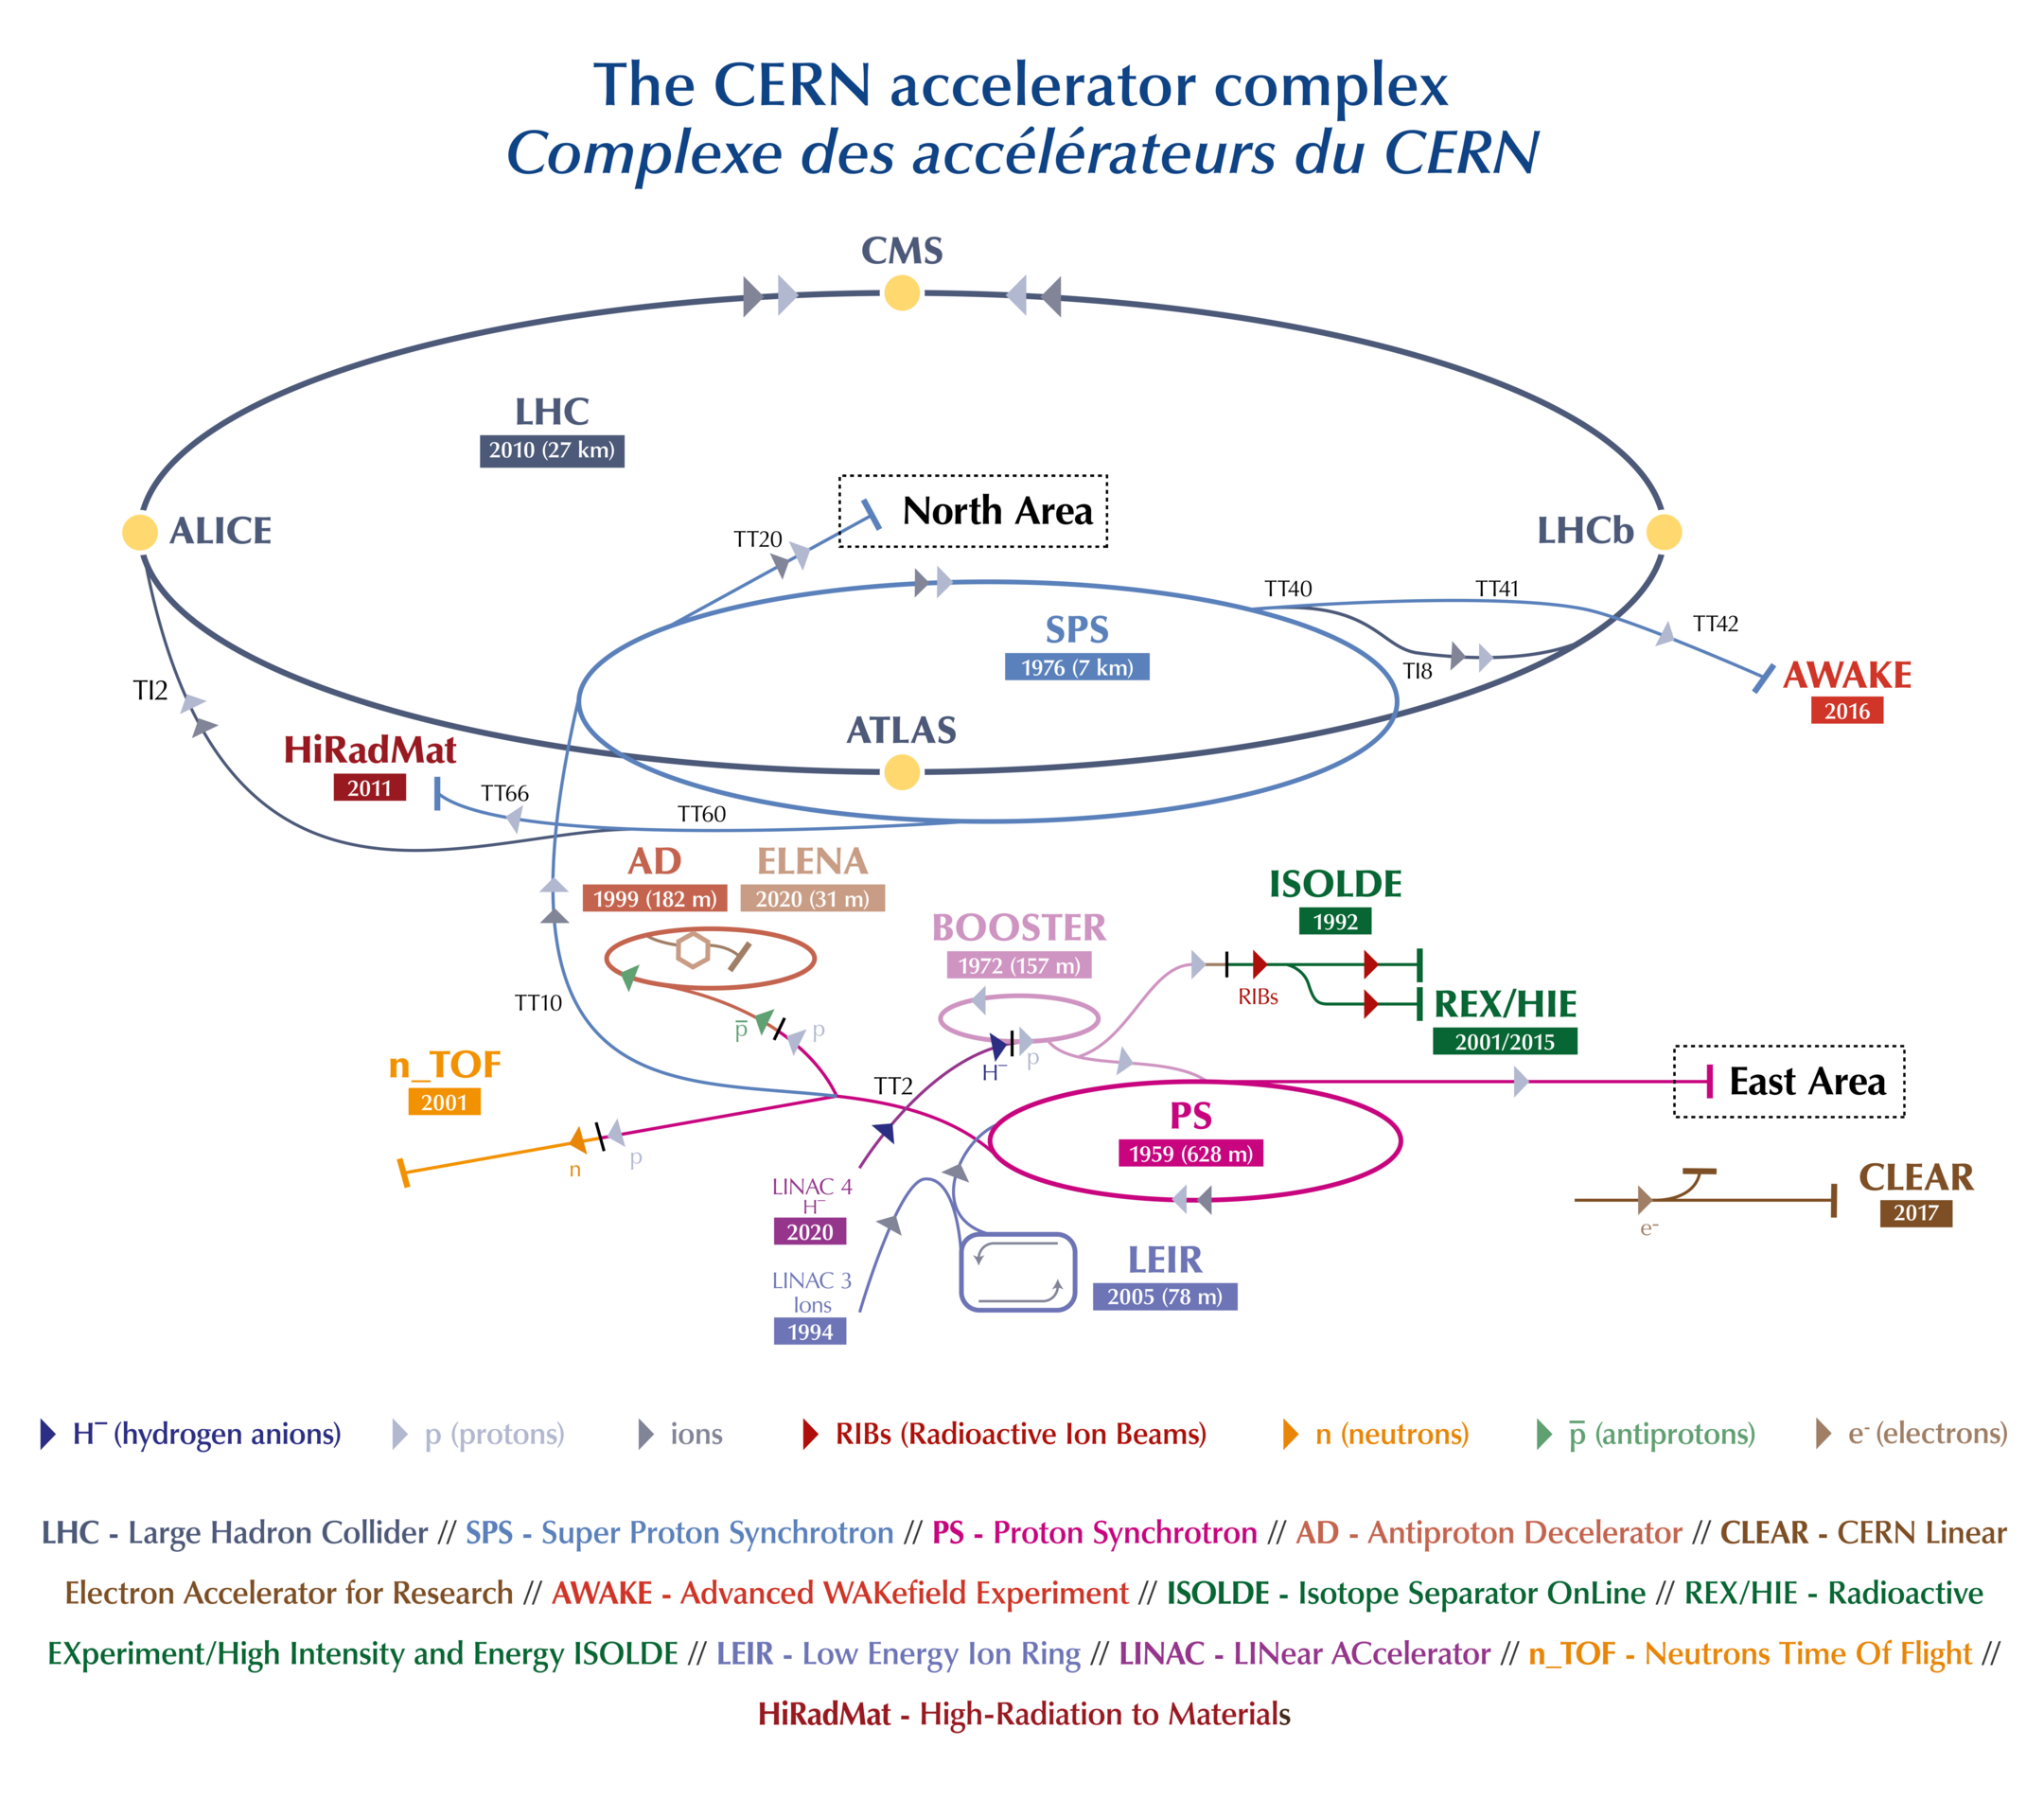
\includegraphics[width=0.75\paperwidth]{CCC-2019}}
	\caption{CERN Accelerators complex \cite{Mobs:2684277}}
\end{figure}

\section{Common Probability Distributions in Physics}
\label{distributions1}

Many problems in physics are described or can be approximated by a small group of probability distributions. In this section, we will briefly describe them \cite{leo2012techniques}.

\subsection{Binomial}

When a problem involve repeated, independent trials with two possible outcomes, the probability is given by the binomial distribution:

\begin{equation}
	P(r)= \frac{N! }{ r! \left( N-r \right)! } p^r (1-p)^{N-r}
\end{equation}

where $p$ is the probability of success in a single trial.

Mean:

\begin{equation}
	\mu = \sum_{r}rP(r) = Np
\end{equation}

Variance:

\begin{equation}
	\sigma^2=\sum_r(r-\mu)^2P(r) = Np(1-p)
\end{equation}

For many practical calculations \cite{leo2012techniques}, using a Gaussian is a good approximation of a Binomial when $N$ is greater than 30 and $p\geq0.05$ (taking into consideration that we are replacing a discrete distribution by a continuos one). If $p$ is small such that the product $Np$ is finite, we can use a Poisson distribution.

\subsection{Poisson}

When the probability is very small ($p \rightarrow 0$) and the numer of trials approaches infinite ($N \rightarrow \infty$) such that the mean $\mu = N p$ remains finite, the \textit{Poisson} distribution occurs:


\begin{equation}
	\label{eqn:poisson}
	P\left( r \right) = \frac{{\mu^{ r } e ^{-\mu} }}{{r!}}
\end{equation}

If the mean is expressed as the mean per unit dimension ($\mu = \lambda t$) we can rewrite \ref{eqn:poisson} as:

\begin{equation}
	P\left( x \right) = \frac{(\lambda t) ^r {e^{ - \lambda t}} }{{r!}}
\end{equation}

\begin{figure}
	\centerline{
		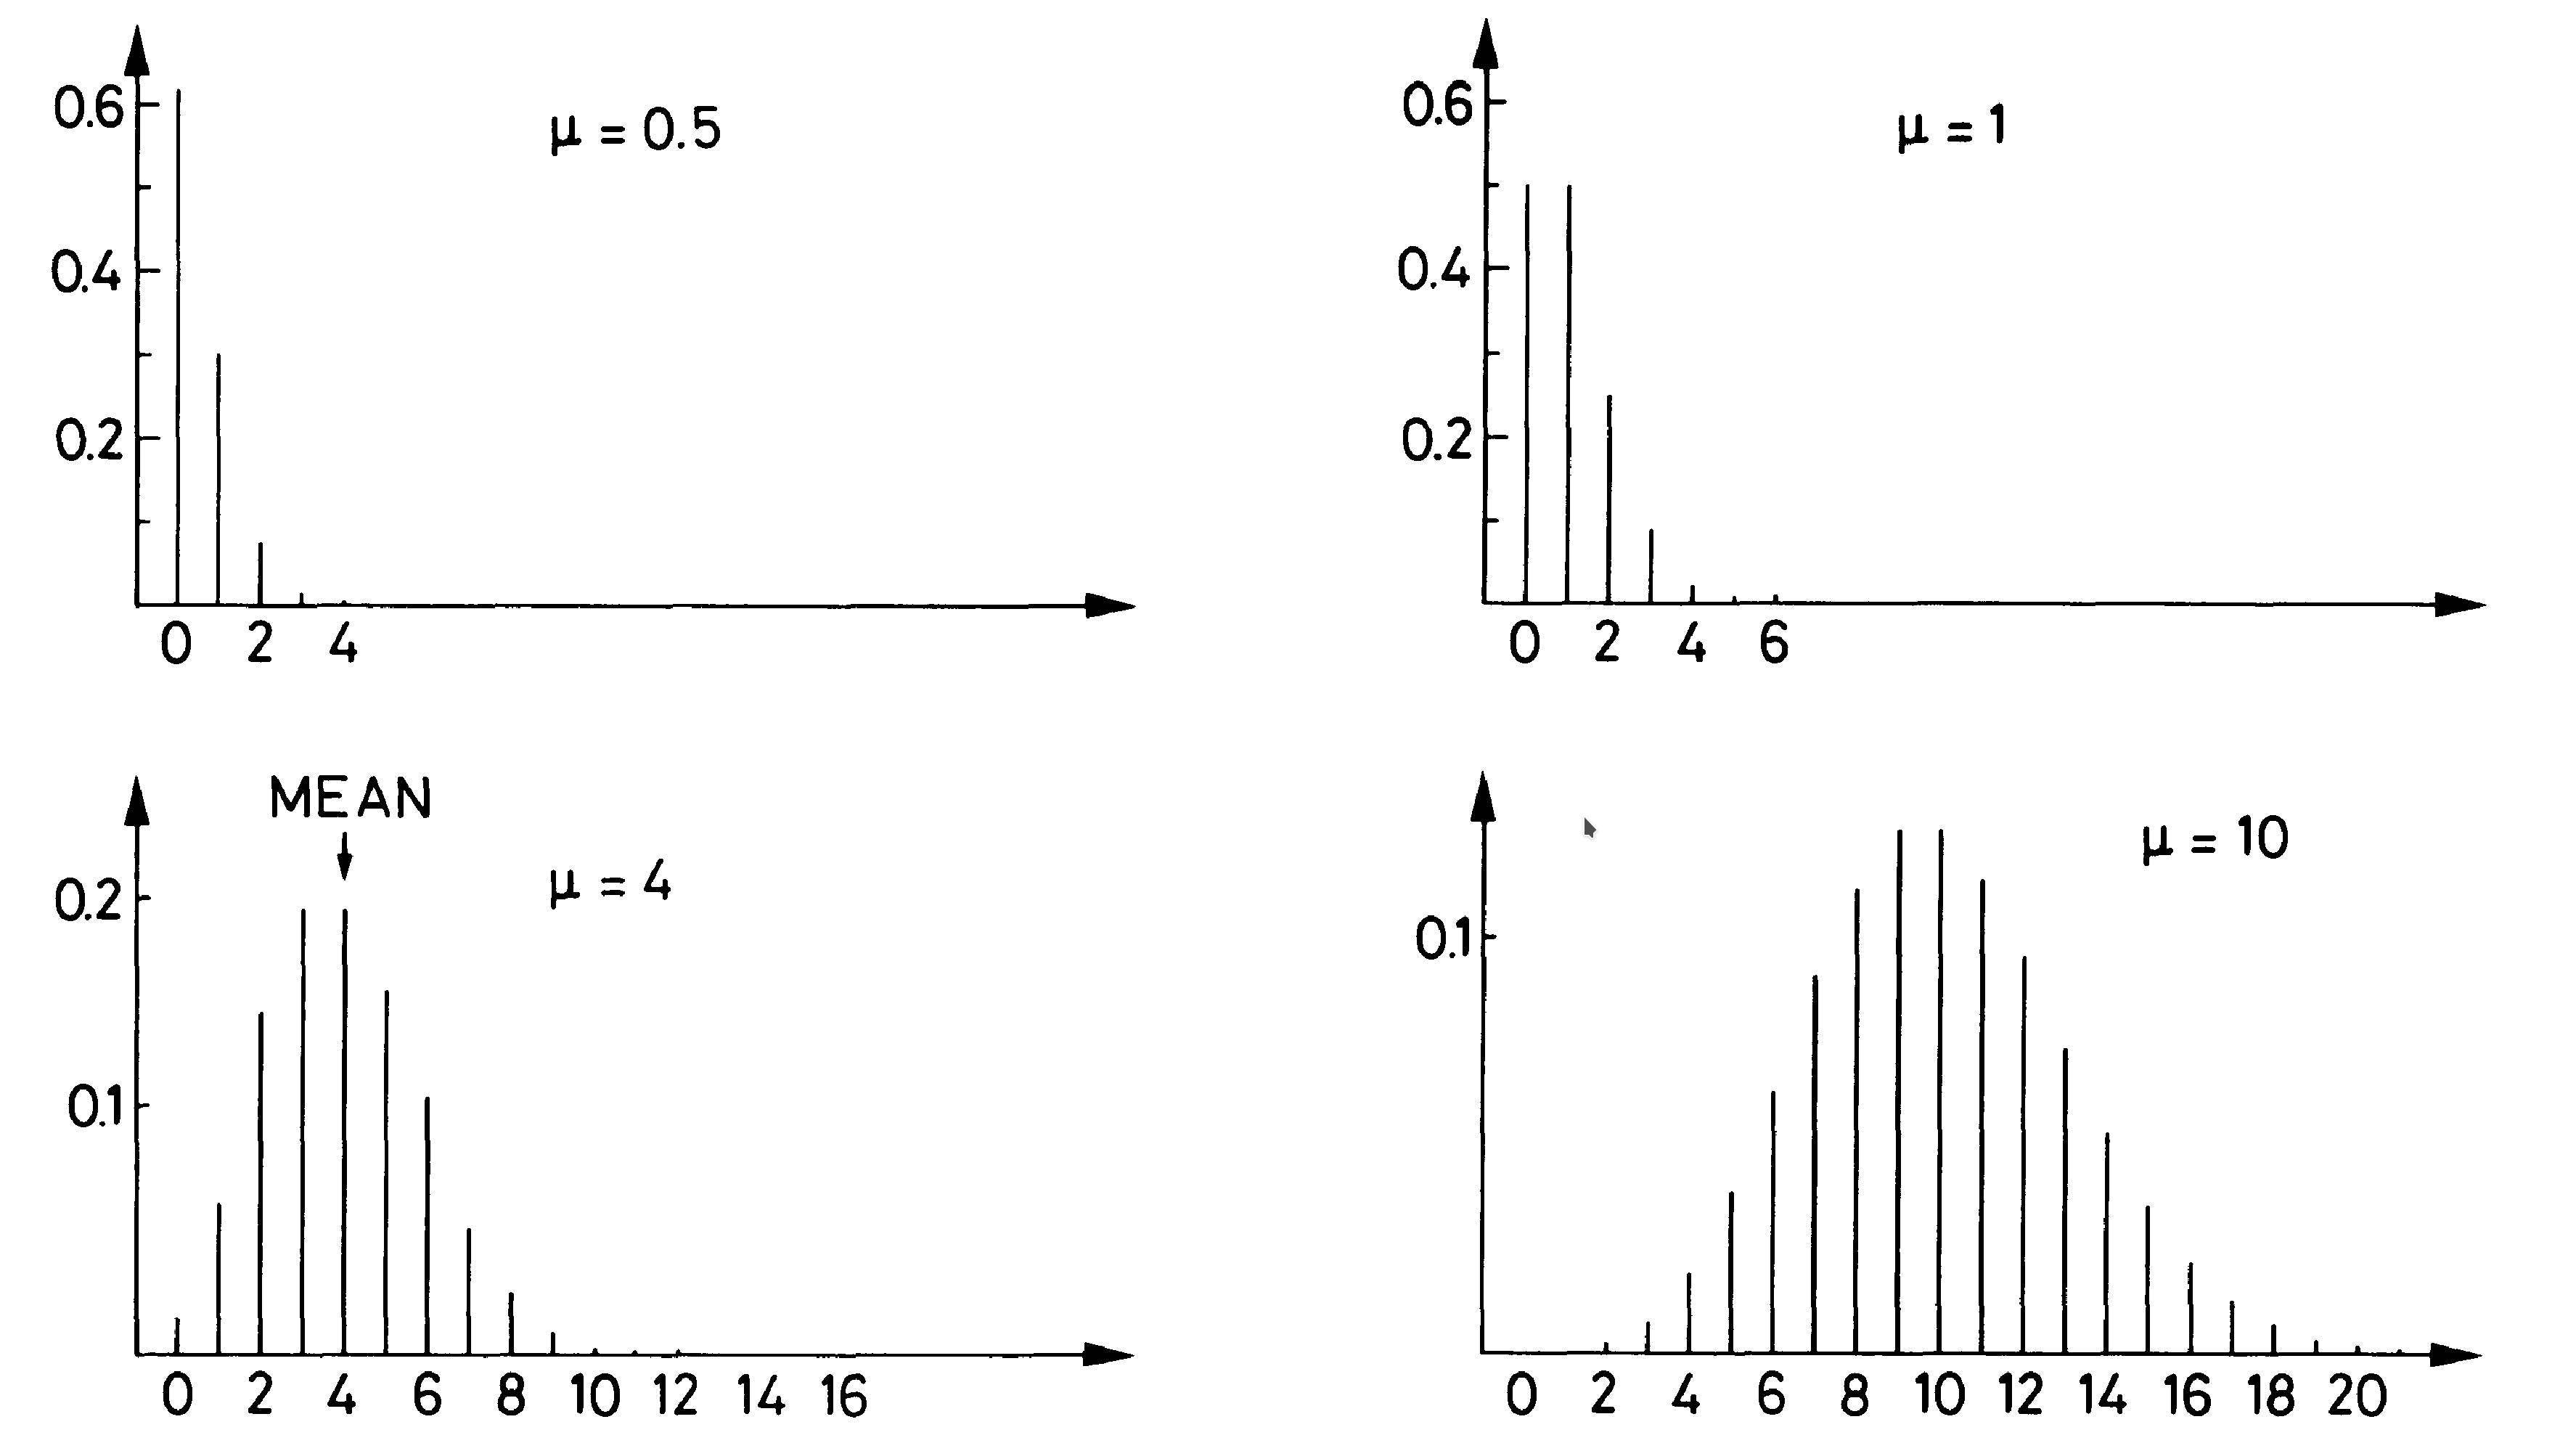
\includegraphics[width=0.5\paperwidth]{poisson}}
	\caption{Poisson distribution with various values of $\mu$ \cite{leo2012techniques}}
\end{figure}

As an example, consider the \textit{radioactive decay} phenomena: a radioactive source such as $^{137}$Cs has a half-life of 27 years. The probability for a single nucleus to decay is $8.2 \times 10^{-10}s^{-1}$. However, even a \SI{1}{\micro\gram} contains $10^{15}$ nuclei. Since each nucleus acts as a \textit{trial}, the mean number of decay events will be $\mu = N p = 8.2 \times 10^5$, satisfying the limiting conditions. The probability of observing an event is given by \ref{eqn:poisson}.

The Poisson distribution exhibits two interesting features:

\begin{enumerate}
	\item Only mean appears, so the knowledge of $N$ and $p$ is not always required. E.g. this happens in experiments involving particle reactions where the mean counting rate is known, rather than the number of particles in the beam.

	\item This distribution only depends on one parameter: $\mu$. We can arbitrarily increase this value by repeating the experiment for higher values of $N$.
\end{enumerate}

\subsection{Gaussian}

The \textit{Gaussian} (or \textit{Normal}) is a continuos, symmetric distribution. Density is defined as

\begin{equation}
	P(x) = \frac{1}{{\sigma \sqrt {2\pi } }}e^{{{ - \left( {x - \mu } \right)^2 } \mathord{\left/ {\vphantom {{ - \left( {x - \mu } \right)^2 } {2\sigma ^2 }}} \right. \kern-\nulldelimiterspace} {2\sigma ^2 }}}
\end{equation}

Where $\mu$ is the mean and $\sigma ^2$ corresponds to the variance. The case where $\mu = 0$ and $\sigma = 1$ is called the \textit{standard} normal distribution.

\begin{equation}
	y = \frac{e^{ - \frac{{x^2 }}{2}}}{{\sqrt {2\pi } }}
\end{equation}

Any Gaussian distribution can be transformed to this reduced form trivially:

\begin{equation}
	z = \frac{x-\mu}{\sigma}.
\end{equation}

\begin{figure}
	\centerline{
		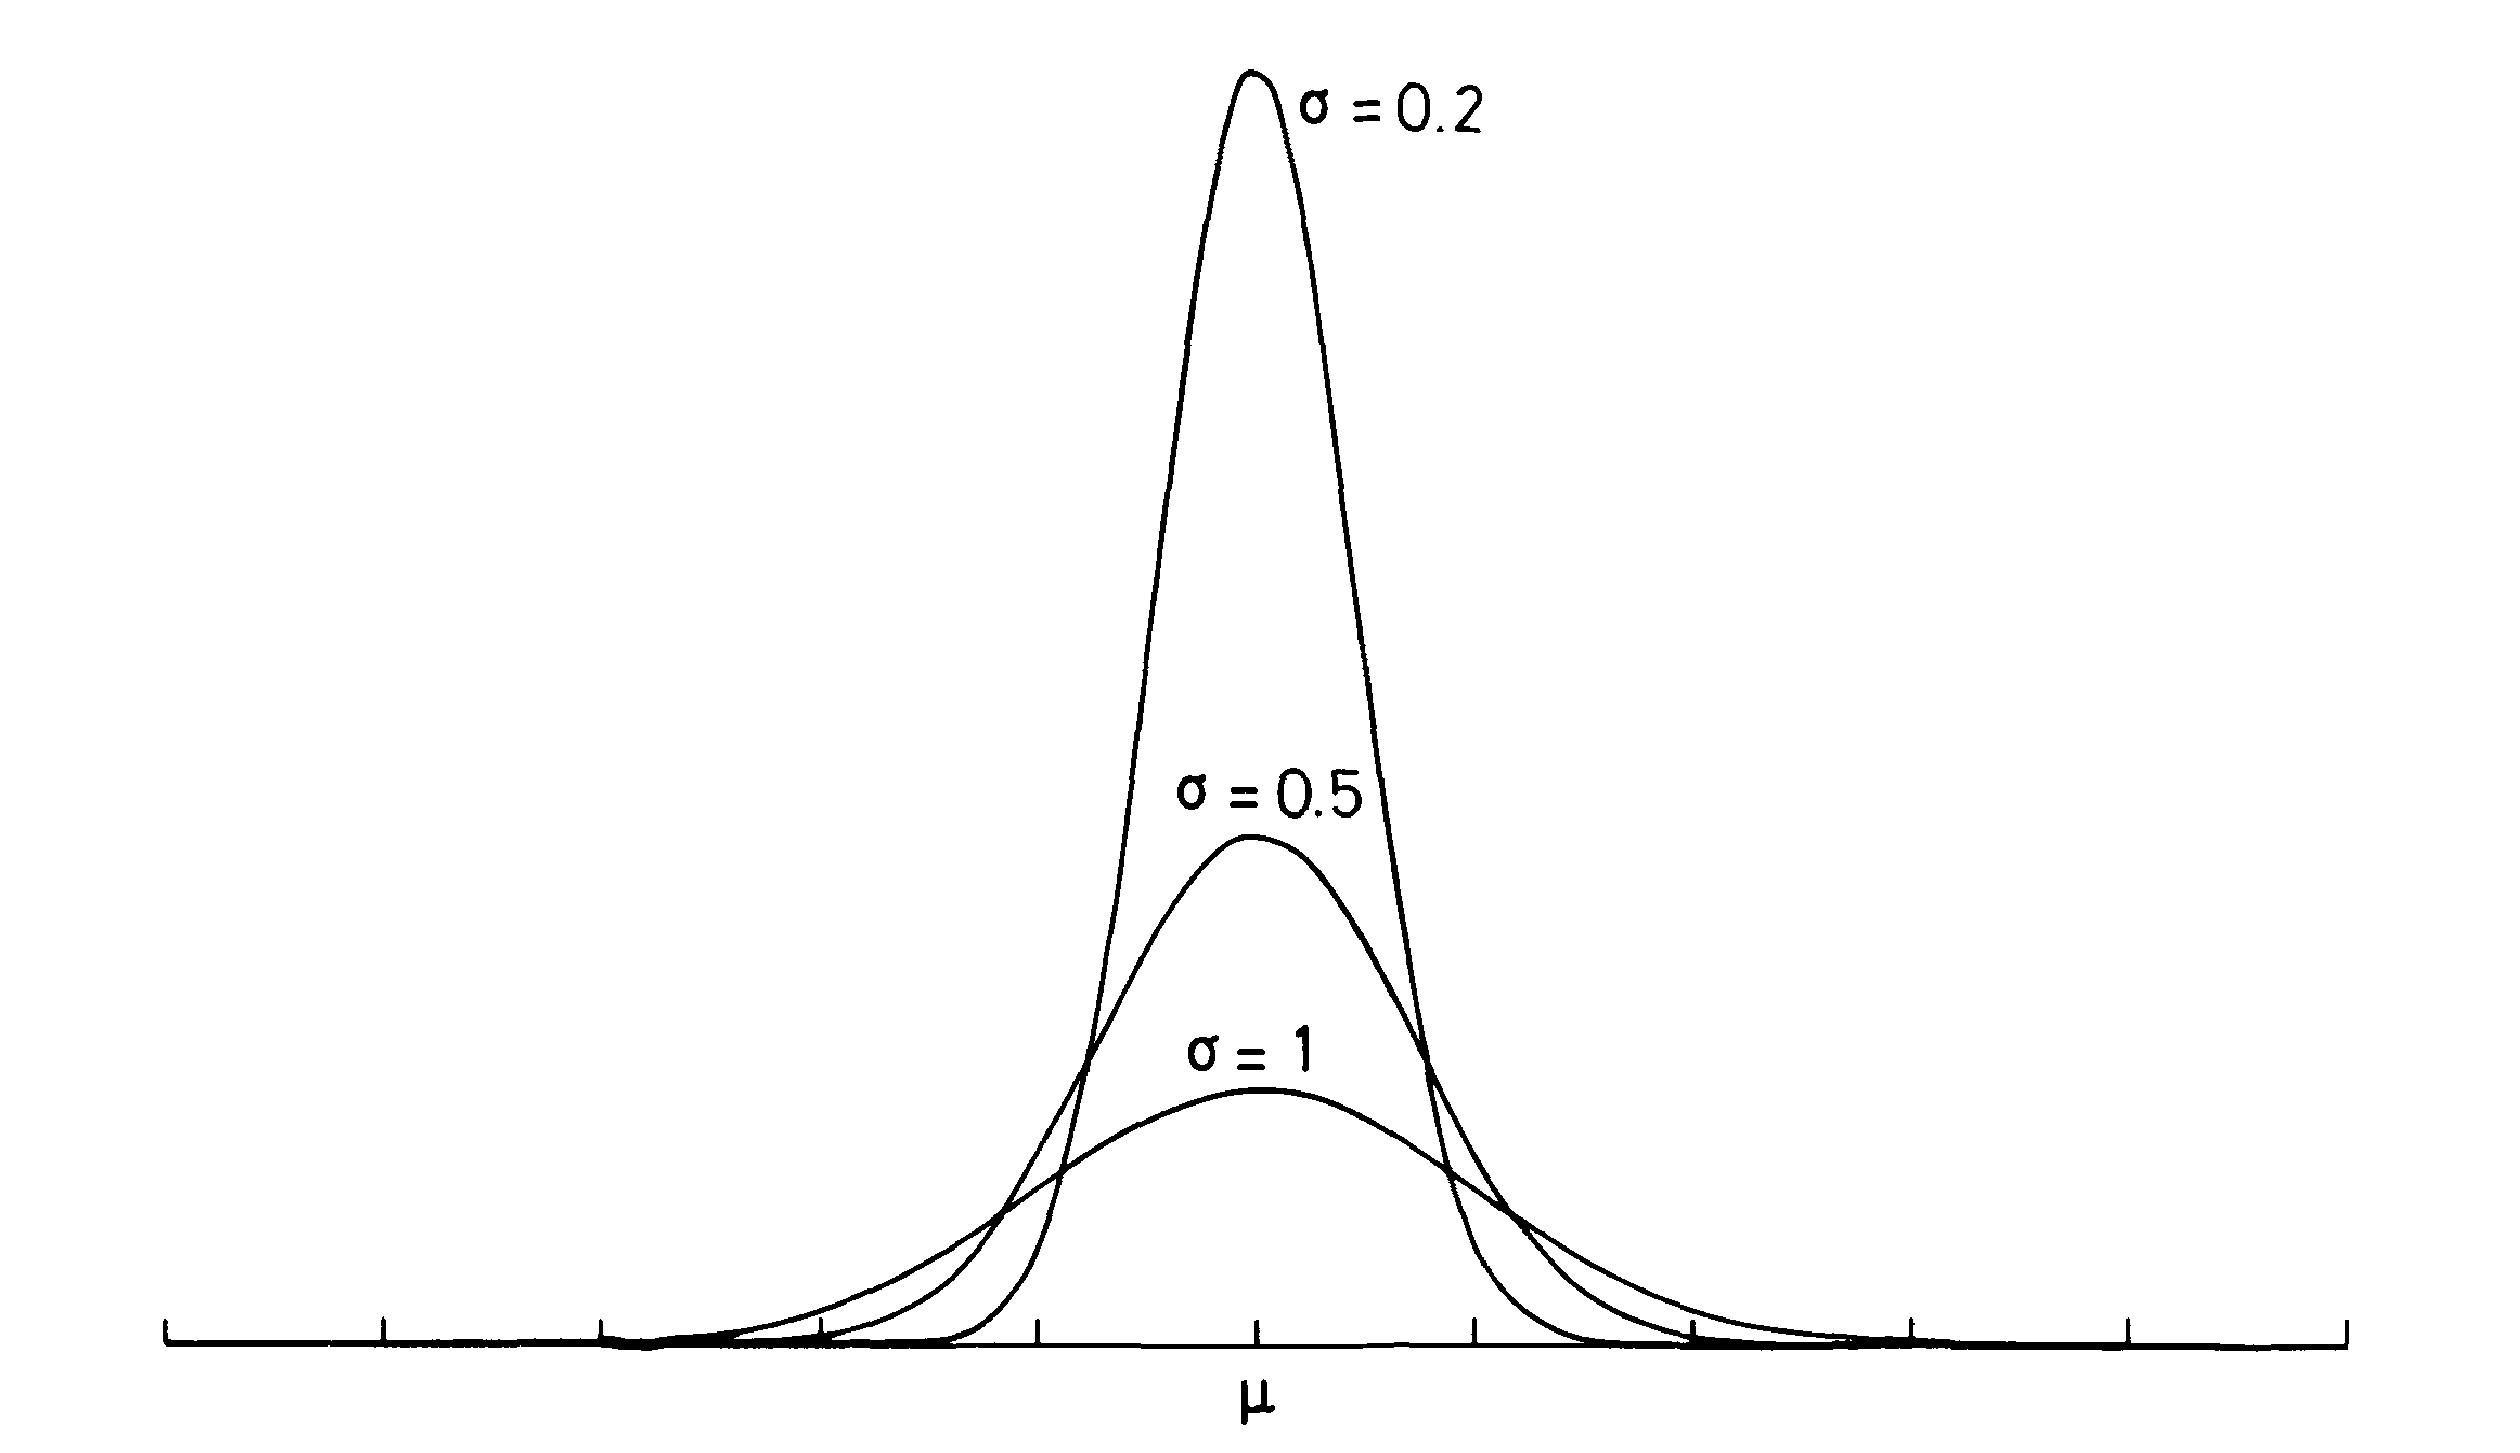
\includegraphics[width=0.5\paperwidth]{gaussian}}
	\caption{Gaussian distribution with various values of $\sigma$ \cite{leo2012techniques}}
\end{figure}

\section{CERN and the LHC}

High Energy Physics experiments need to collect a large quantity of data to attack the statistical nature of particle physics and find interesting and rare phenomena with enough accuracy.

While Systematic Errors are harder to handle, uncertainties caused by Random Errors follow known distributions (like a Poisson rate) or are empirically determined. As we've seen \ref{distributions1}, repeating measurements provides larger samples to estimate these uncertanties and get more accurate data.

\subsection{Cross Section}

Cross section ($\sigma$) is one of the most important quantity in particle physics: it measures the probability than a specific process occurs in a collision of two particles. It is expressed in terms of the transverse area that the particle must hit to for that process to occur and it's measured in \textit{Barn}: $1b = 10^{-24} cm^2$.

E.g. the \textit{Rutherford cross-section} represents the probability of an alpha-particle to be deflected by a given angle during a collision with an atomic nucleus.

\subsection{Luminosity}

This value is a measurement of the number of collisions that can be produced in a detector (point of collision) per $cm^2$ and per second. It can be calculated in this way:

\begin{equation}
L\sim \frac{N^2}{t S_{\text{eff}}}
\end{equation}

Where $t$ is time between bunches, $S_{\text{eff}} = 4 \pi \sigma^2$ is the section offective of collision. In LHC, $\sigma = 16\times 10^{-4} cm$.

\section{CMS}

\section{CMS Trigger System}


The LHC generates 40 milions events per second. Each CMS event, on average, carries a payload of 1 MB of unprocessed informations. It is technologically impossible to retain this amount of data, due to hardware, software, network and storage constraints.

Furthermore, most events represent uninteresting information for the current state of physics knowledge.

The \textit{CMS Trigger System} is designed to reduce the output stream to 1000 events per second, while preserving the physics reach of the experiment.
It is composed by a hierchical set of rules, called Trigger Nodes (or Paths): each one probes a specific patterns (physics signature) in the event or looks for specific physics objects.

This happens in two steps:

\begin{enumerate}

	\item The first level (L1) \cite{Bayatyan:706847} brings the 40 MHz to a 100 kHz rate. Here, N Trigger Algorithms are implemented on custom electronics (FPGAs and ASICs) exploiting informations from sub-detector components.

	\item A configurable set of L1 Trigger Nodes seeds Triggers in the second level (HLT), implemented in software. The event stream is further refined, selecting an average rate of 400 Hz for offline event storage and certification \cite{Khachatryan_2017}. HLT runs 600 of these independent Trigger Paths.

\end{enumerate}